\section{Detailed results}
\label{detailedresults}

\subsection{Functional tests}
The main purpose of the functional testing is to ensure the correctness of the transport
calculation functions of the code.

\subsubsection{7.2.1.1 Neutron/Photon flux}
Test case: Calculate the spectra distribution in three locations in ITER tokamak (e.g.
equatorial inboard and outboard blankets, divertor region including TFC leg) as
specified in reference. The energy bins for comparing spectra are reported in Tab.1.
The calculation should be performed based on the ITER C-lite model or reference
models released after C-lite.

Test method: The code should provide geometry visualization method using the ray
tracing method as same as that used in the nuclear transport simulation. First compare
the geometry visualized by the code with the anticipated geometry, if it passes the
comparison, it would verify the correctness of the complex geometry used for the
transport simulation of the code. Then compare the calculation results with those
calculated by the reference code (such as MCNP), accept the calculation results as
correct if they conform the acceptance criterial described in section 7.3.

\subsubsection{7.2.1.2.1 Nuclear heat}
Test case: Calculate the nuclear heat deposition on a number of specific locations
including the first wall (FW), blanket (BLK), vacuum vessel (VV), TF coil (TFC) and
divertor for a number of the specific materials separately for neutron and photon in the
specific energy bin structures. Table 2 shows the materials, location and energy bin
structure for this calculation. The calculation should be performed based on the ITER
C-lite model or reference models released after C-lite.

Test method: Compare the calculation results with those calculated by the reference
code (such as MCNP), accept the calculation results as correct if they conform the
acceptance criterial described in section 7.3.

\subsubsection{7.2.1.2.2 Tritium Production Rate}
Test case: HCPB.

Test method: Compare the calculation results with experiment measurements (The
positions are POS 4,6,8 in HCPB model), accept the calculation results as correct if
they conform the acceptance criterial described in section 7.3.

\subsubsection{7.2.1.2.3 Dose}
Test case: FNG/dose.

Test method: Compare the calculation results with experiment measurements (The
decay time are 15,30,60 days) or the results calculated by the reference code (such as
MCNP), accept the calculation results as correct if they conform the acceptance criterial
described in section 7.3.

\subsubsection{7.2.1.2.4 Helium production rate}
Test case: FNG-BLKT.

Test method: Compare the calculation results with experiment measurements or the
results calculated by the reference code (such as MCNP), accept the calculation results
as correct if they conform the acceptance criterial described in section 7.3.

\subsubsection{7.2.1.2.5 DPA}
Test case: DT-FW. \textit{Model could not be provided by the IO or retrieved from anywhere. The IO agreed C-model can be used.}

Test method: Compare the calculation results with those calculated by the reference
code (such as MCNP), accept the calculation results as correct if they conform the
acceptance criterial described in section 7.3.

\subsection{Fundamental tests}
The main purpose of this testing is to verify the implementations of the Monte Carlo method
and the preservation laws.

\subsubsection{7.2.2.1 Test of statistical error}
Purpose: To verify the trend and correctness of statistical error.

Test case: The model is a simple vacuum sphere with radius 5 cm, and the isotropic
neutron source is defined in the position 10 cm from the centre of the sphere with mono
energy 14MeV. The neutron flux in the sphere is counted for different particle histories.

Test method: Perform three independent calculations with increasing 10,000, 100,000
and 1,000,000 particle histories. Compare the trend of the statistical error, check if the
values decrease linearly with the square root of the history number. And then compare
the statistical errors of neutron flux in the vacuum sphere with the theoretical value as 
\textit{TEXT MISSING IN ORIGINAL DOCUMENT. 
From context, the continuation of the sentence was assume to be: the inverse square root dependence on the number of particle histories.}

Problem was setup as described and ran with OpenMC. Results:
\begin{figure}[H] 
	\centering 
	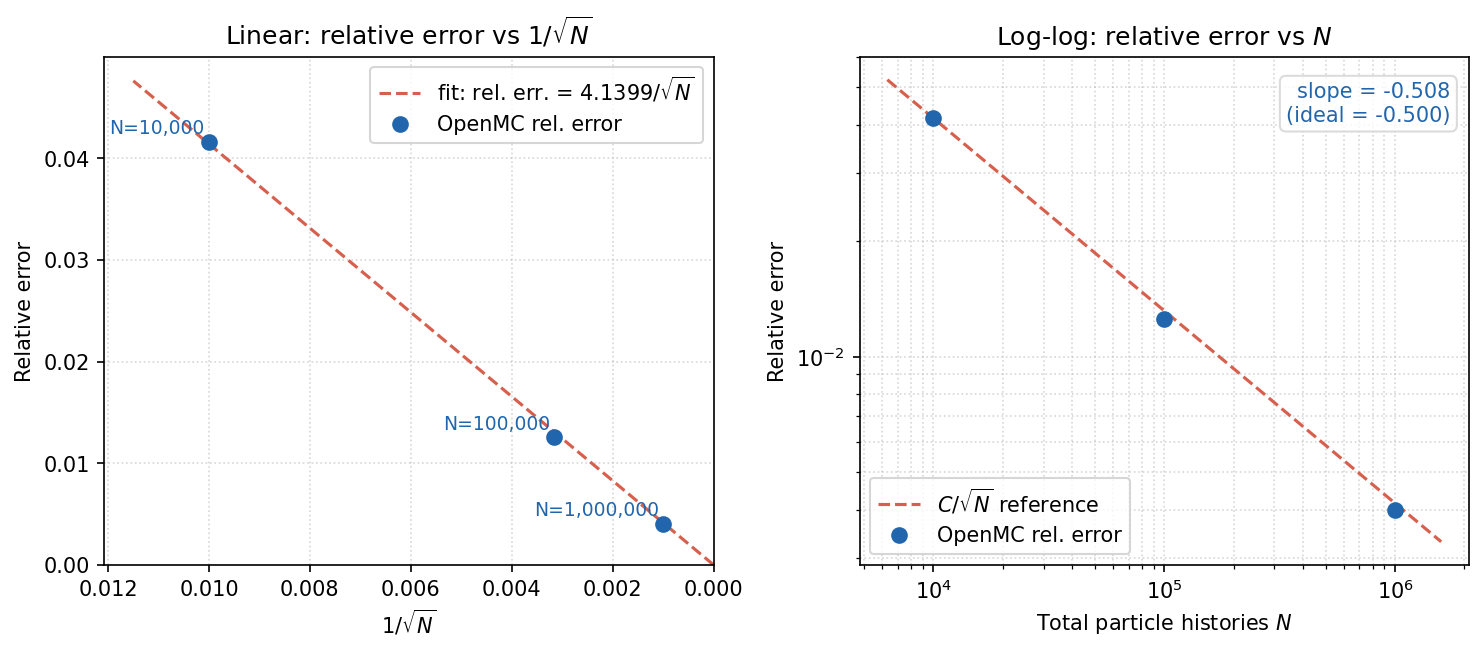
\includegraphics[width=0.95\textwidth]{../fundamental_testing/7221_se/7221_se_1.png} 
	\caption{Statistical convergence of results as a function of increasing simulated particle histories.} 
	\label{fig:7221-1} 
\end{figure}

\subsubsection{7.2.2.2 Test of statistical error with weight window}

Purpose: To verify the trend and correctness of statistical error with/without weight
window variance reduction techniques.

Test case: The models of the variance reduction examples.
Test method:Perform several independent calculations with increasing particle
histories 10,000, 100,000 and 1,000,000 with and without use of the variance reduction
technique(s). Then compare the trend of the statistical errors, check whether the
statistical error with variance reduction on is smaller than that without use of the VR
technique at the same histories. When calculating with a weight window, the variance
of the variance should be calculated, to verify the convergence of the calculation
results. Only results with the expected behaviour of the mean, variance, and the
variance of the sample variance should be considered valid for the statistical error test.

Problem was setup as described in and ran with OpenMC. The model is a simple concrete cube (2 m sides) with a 14 MeV neutron source. 
The qunatites of interst are tallies in cells at increasing shield thicknesses in 10 cm increments. The Random-Ray solver is used to create FW-CADIS based weight windows on the fly. Results:
\begin{figure}[H] 
	\centering 
	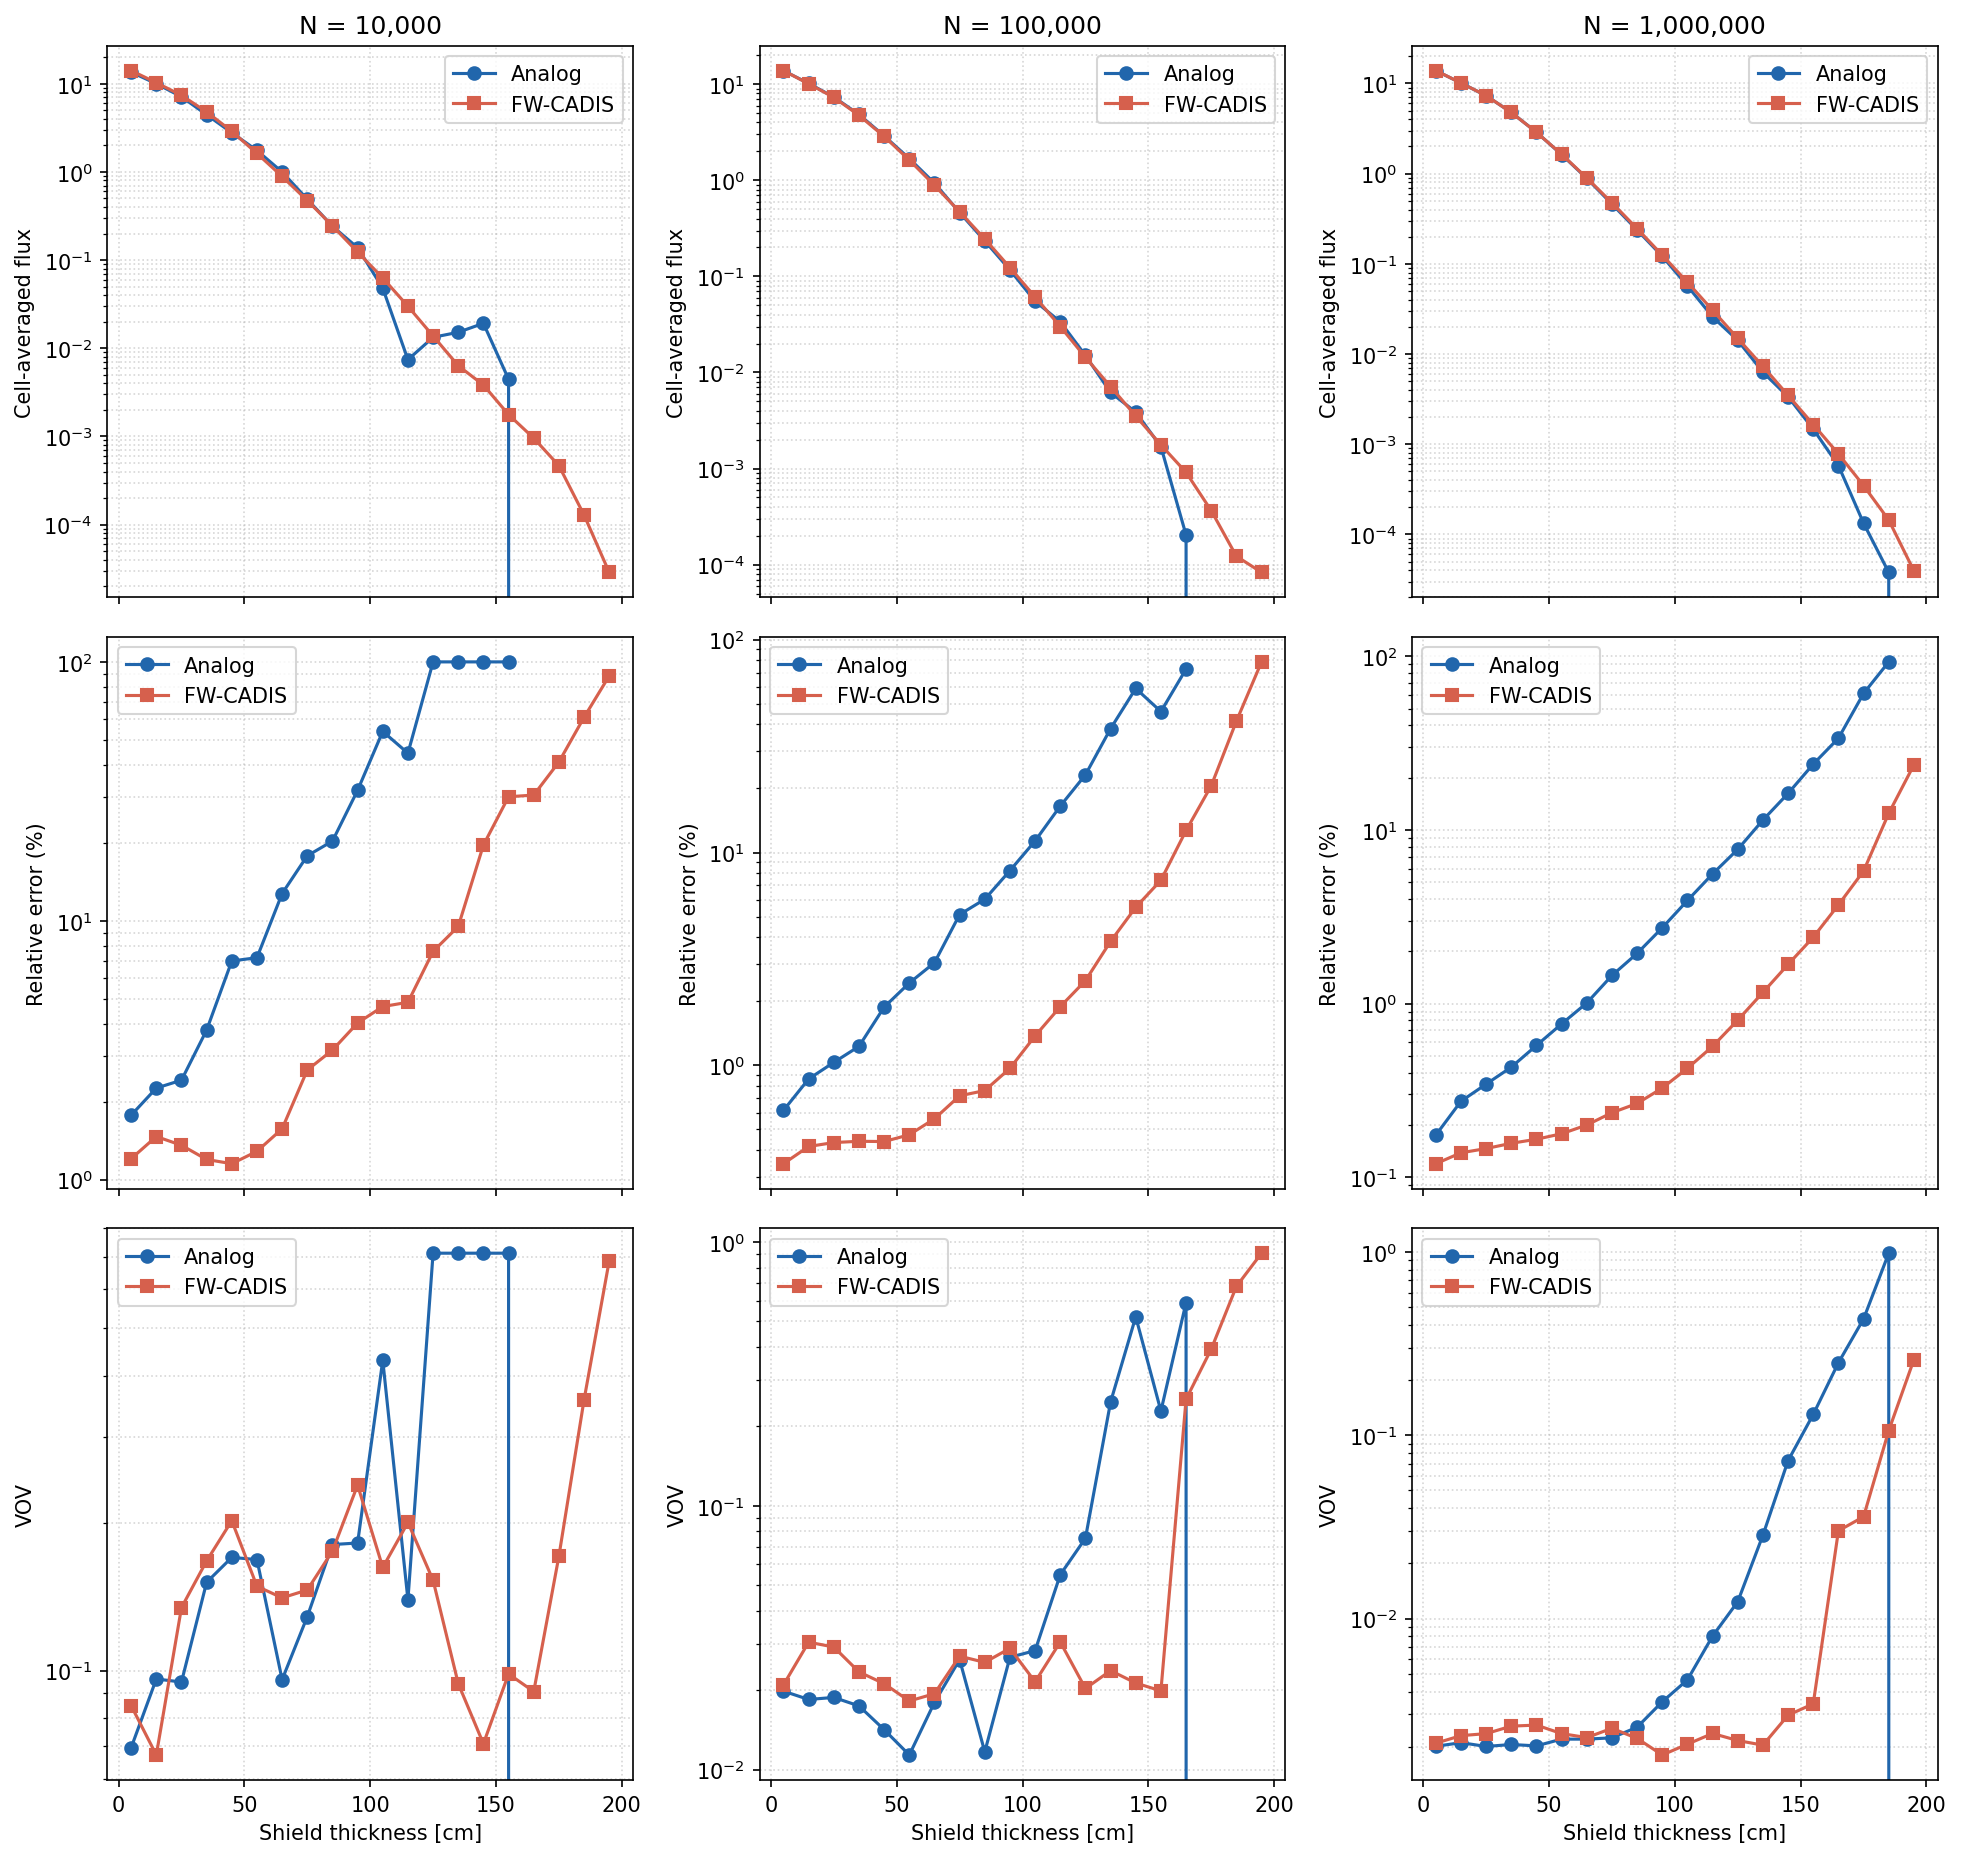
\includegraphics[width=0.95\textwidth]{../fundamental_testing/7222_seww/7222_seww_1.png} 
	\caption{Comparisson of analog and weight window accelerated simulation result as a function of shield thickness. Each colum represent a 10-fold increase in simulated particle histories.  Top row mean results, middle row relative error, bottom row Variance of Variance.} 
	\label{fig:7222-1} 
\end{figure}

\subsubsection{7.2.2.3 Test of random number generator}
Purpose: To verify the correctness of the random number generator. As random
number generators in Monte Carlo codes are implemented based on LCGs, this test is
aiming to verify the correctness of the LCGs implemented in the code.

Test case 1: The standard statistical tests for random number generators described by
Knuth or variations on Knuth's statistical tests.

The problem was setup as described. The random number generator was accessed via the DLL. A series of tests were run including:
Frequency, Serial, Runs, Gap, Poker, Autocorrelation.
For more details you can look at the full test report in: \path{/fundamental_testing/7223_rng/1} of the
\href{https://github.com/openmc-dev/openmc-fundamental-testing}{OpenMC Fundamental Testing git repository}.
\vspace{0.5em}
Test case 2: Marsaglia's DIEHARD test suite for random number generators.

Test Method: Write random stream generating program based on the LCGs code
implemented in the code. Apply the two test cases to the random stream generated by
the random stream generating program, if it passes the acceptance criteria, the random
number generator of the code can be considered as acceptable.

The problem was setup as described. The random number generator was accessed via the DLL. The Diehard test suite was run using the the modern implementation as part of Dieharder.
Diharder can be installed from the \href{https://github.com/seehuhn/dieharder}{Dieharder git repository} or in Ubuntu/Debian simply by \verb|sudo apt-get install dieharder|.

List of tests performed:
\begin{itemize} 
\item Birthday Spacings Test -- \verb|-d 0| (Diehard Birthdays Test) 
\item Binary Rank 31x31 and 32x32 -- \verb|-d 2| (Diehard 32x32 Binary Rank Test)
\item Binary Rank 6x8 -- \verb|-d 3| (Diehard 6x8 Binary Rank Test)
\item Bitstream -- \verb|-d 4| (Diehard Bitstream Test) 
\item OPSO (Overlapping-Pairs-Sparse-Occupancy) -- \verb|-d 5| (Diehard OPSO Test) 
\item OQSO (Overlapping-Quadruples-Sparse-Occupancy) -- \verb|-d 6| (Diehard OQSO Test) 
\item DNA -- \verb|-d 7| (Diehard DNA Test) 
\item Count the 1s (stream of bits) -- \verb|-d 8| (Diehard Count the 1s Stream Test) 
\item Count the 1s (specific byte) -- \verb|-d 9| (Diehard Count the 1s Byte Test) 
\item Parking Lot Test -- \verb|-d 10| (Diehard Parking Lot Test) 
\item Minimum Distance (2D circles/spheres) -- \verb|-d 11| (Diehard Minimum Distance Test) 
\item 3D Spheres (Minimum Distance) -- \verb|-d 12| (Diehard 3D Sphere Test) 
\item Squeeze Test -- \verb|-d 13| (Diehard Squeeze Test) 
\item Runs Test (Wald-Wolfowitz) -- \verb|-d 15| (Diehard Runs Test) 
\item Craps Test -- \verb|-d 16| (Diehard Craps Test) 
\end{itemize}

For more details you can look at the full test report in: \path{/fundamental_testing/7223_rng/2} of the
\href{https://github.com/seehuhn/dieharder}{OpenMC Fundamental Testing git repository}.

\subsubsection{7.2.2.4 Test of source sampling}
Purpose: To verify the correctness of the source sampling with probability distribution.

Test case 1: The model is a simple vacuum sphere with radius 5 cm, and the isotropic
neutron source is defined in the centre of the sphere with specific energy distribution.
Tally the neutron energy integrated over the sphere surface with refined energy bins.

Test method 1: Perform calculation until the tally results in each energy bin converge.
Compare the calculation results with the specific energy distribution of the source
definition, consider the code passes this test if the results meet the requirements
described in section 7.3.

Problem was setup as described and ran with OpenMC. A triangular enerrgy distibtuion was chosen. Results:
\begin{figure}[H] 
	\centering 
	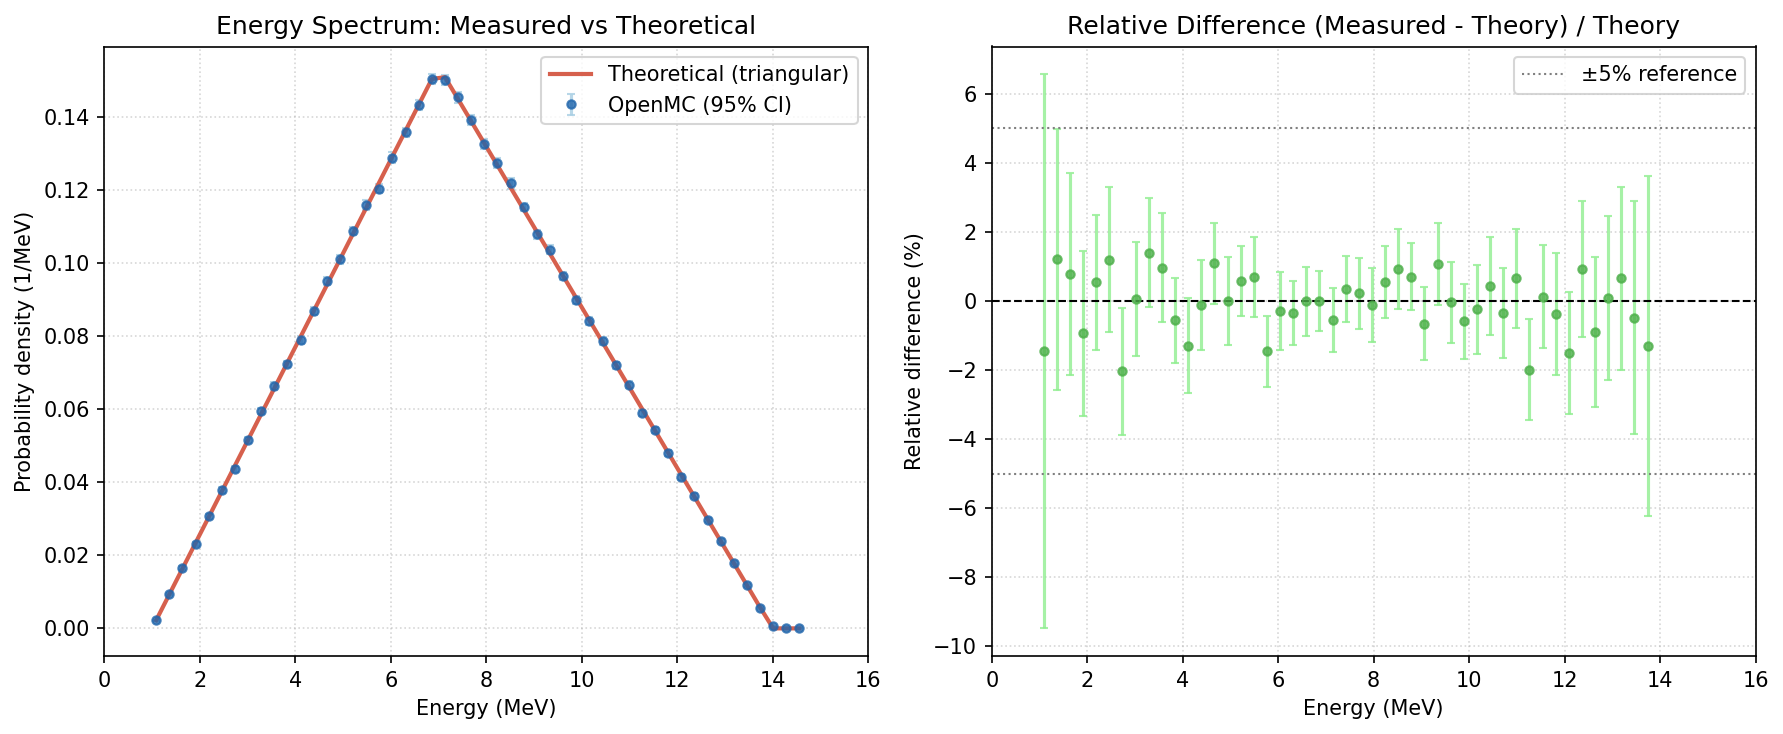
\includegraphics[width=0.95\textwidth]{../fundamental_testing/7224_ss/1/7224_ss_1.png} 
	\caption{Simulated vs theoretical source energy distribution.} 
	\label{fig:7224-1} 
\end{figure}
\vspace{0.5em}
Test case 2: The model is a simple vacuum cuboid pipe with length 10 cm*0.1 cm*0.1
cm (the coordinate of centre point is zero, dimension is defined in the order of x, y, z
axis). The neutron source is defined inside the plate with single direction along the z
axis, and the distribution of the source position is sampled by a specific distribution
along x axis and constant along y and z axis. The surface current of the top surface
(perpendicular to z axis and on the top of the cuboid pipe) segmented evenly to 100
segments by refined surfaces perpendicular to x axis are counted.

Test method 2: Perform calculations until all the tallies in all the segments converge.
Compare the results to the source position sampling, the code would be considered
passed this test if the results meet the criterial described in section 7.3.

Problem was setup as described and ran with OpenMC. A triangular positional distibtuion was chosen. Results:
\begin{figure}[H] 
	\centering 
	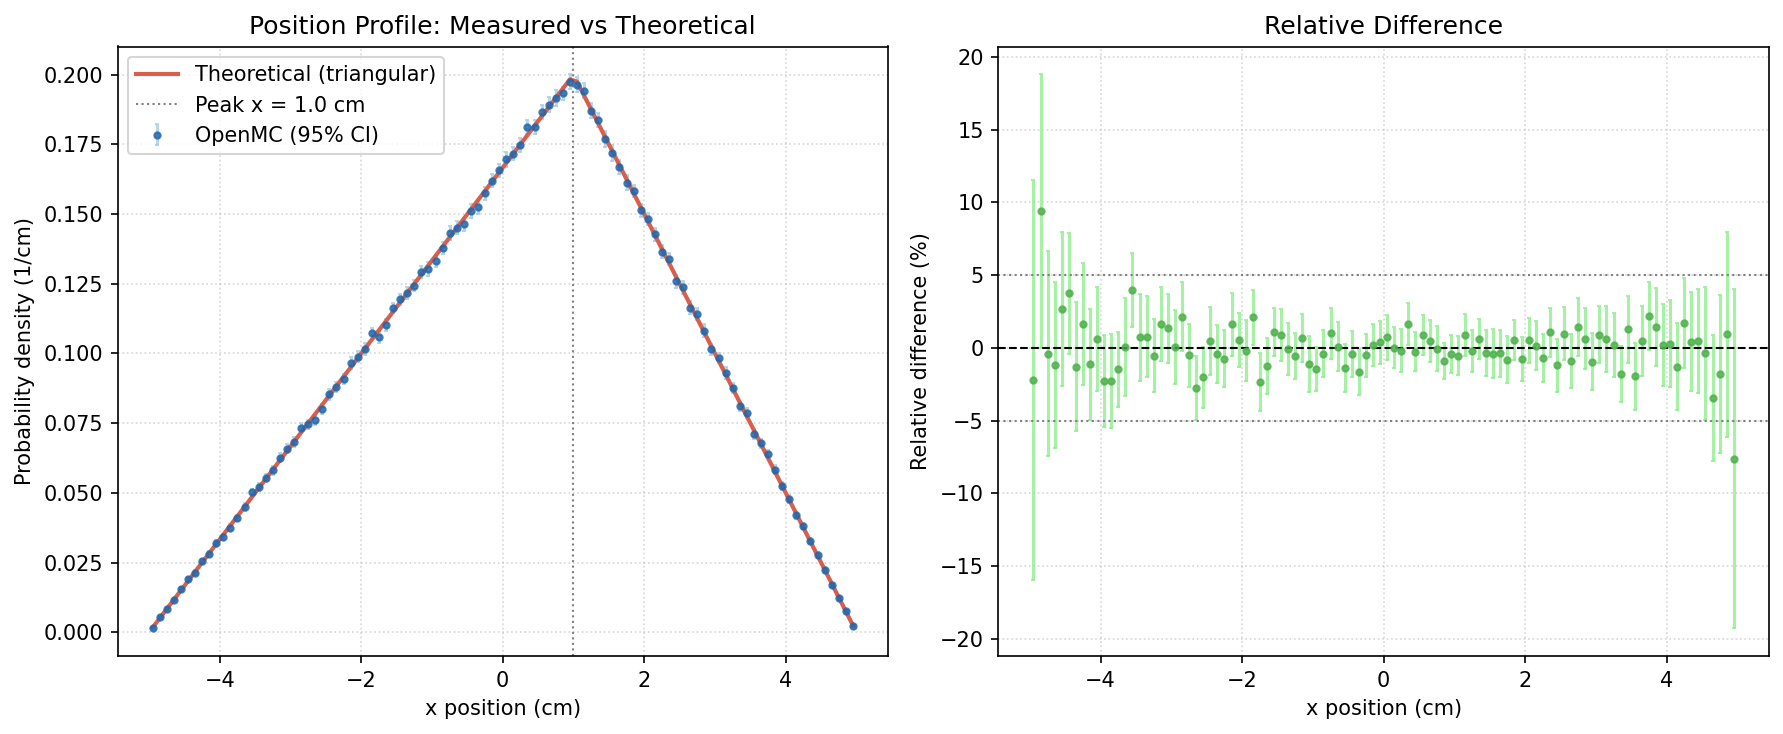
\includegraphics[width=0.95\textwidth]{../fundamental_testing/7224_ss/2/7224_ss_2.png} 
	\caption{Simulated vs theoretical source positional distribution.} 
	\label{fig:7224-2} 
\end{figure}

\vspace{0.5em}
Test case 3: The model is a simple vacuum circular slab with 5 cm radius and 1 cm
thickness along with z axis, and the mono neutron source (14MeV) is defined in the
centre line of the slab with specific direction distribution (perpendicular to z axis with
refined distributions). Split the slab into 365 segments that each segment is reference to
1 degree, and tally the neutron flux in each segment.

Test method 3: Perform calculations until all the tallies in all the source bins converge.
Compare he results to the source direction sampling, the code would be considered
passed that this test if the results met the criterial described in section 7.3.

Problem was setup as described and ran with OpenMC. A sinusioidal non-uniform azimuthal distribution angular distibtuion was chosen. Results:
\begin{figure}[H] 
	\centering 
	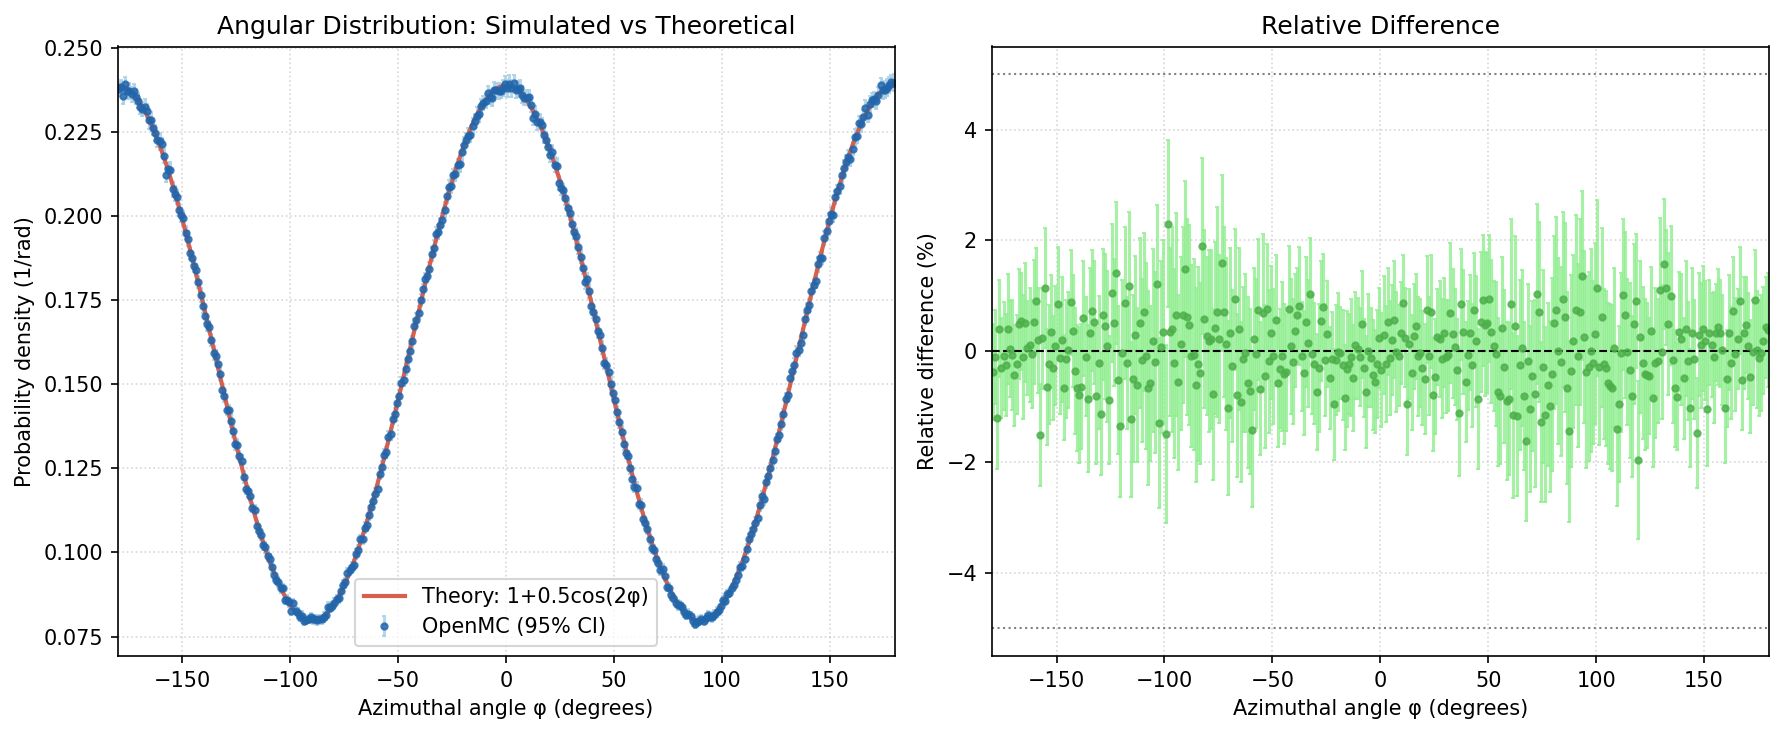
\includegraphics[width=0.95\textwidth]{../fundamental_testing/7224_ss/3/7224_ss_3.png} 
	\caption{Simulated vs theoretical source angular distribution.} 
	\label{fig:7224-3} 
\end{figure}

\vspace{0.5em}
Test case 4and the plasma solid with reflection surfaces is used as the test model. The
neutron flux in the mesh with grid size of 10cm*10cm*10cm covering the C-lite model
would be tallied.

Test method 4: Perform calculations until tallies of all the grids converge, compare the
results with MCNP results, considered the code passed this test if the results meet the
criteria described in section 7.3.

Problem was setup in MCNP and OpenMC according to the description. The ITER C-model plasma source was translated into OpenMC. Both the MCNP and OpenMC plasma source were postioned in to a voided wedge with reflective boundaried. Results:
\begin{figure}[H] 
	\centering 
	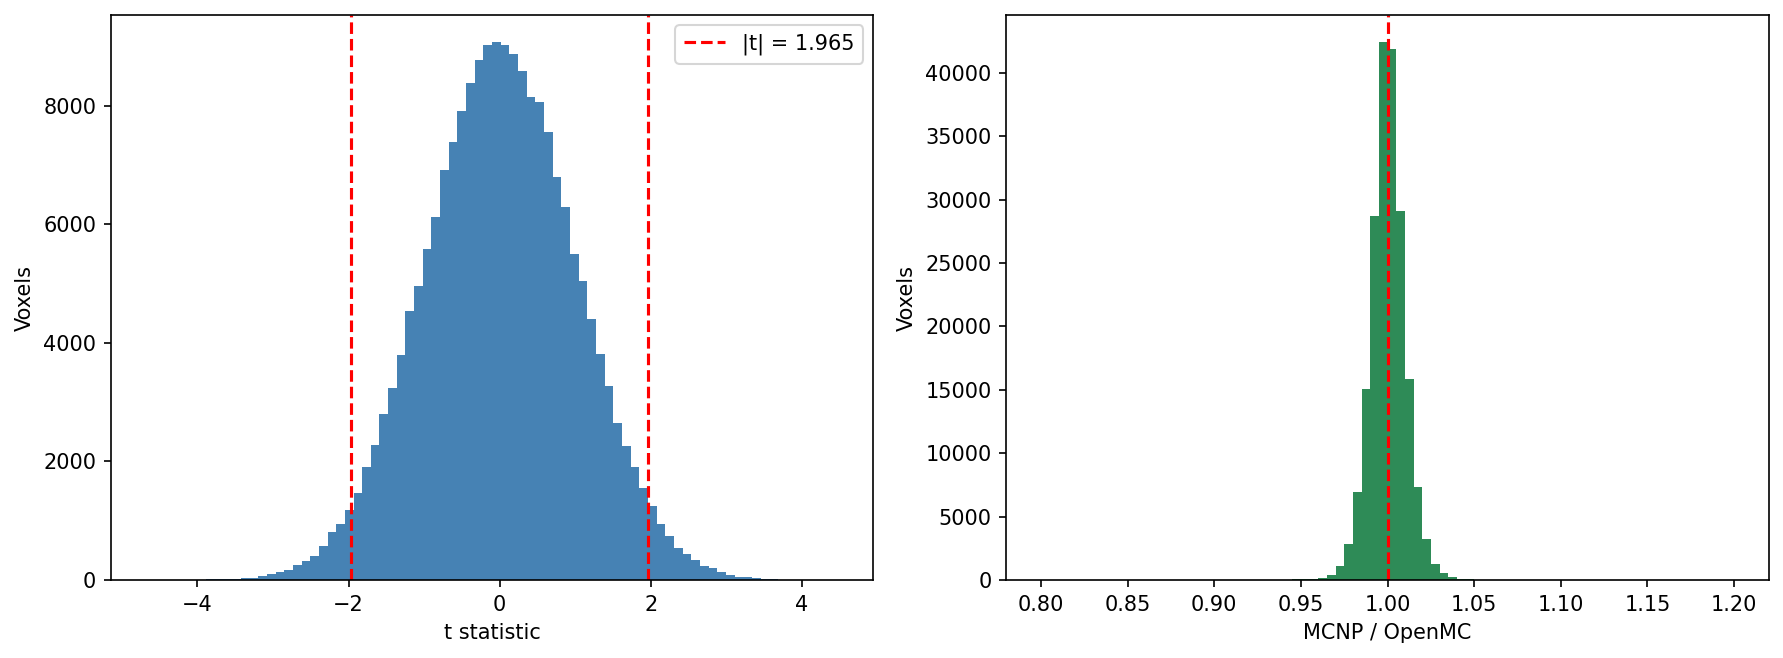
\includegraphics[width=0.95\textwidth]{../fundamental_testing/7224_ss/4/7224_ss_4-TTest.png} 
	\caption{Student t-statisitical test results and ratio of fluxes on a 10cm mesh in MCNP and OpenMC.} 
	\label{fig:7224-4} 
\end{figure}

\begin{figure}[H] 
	\centering 
	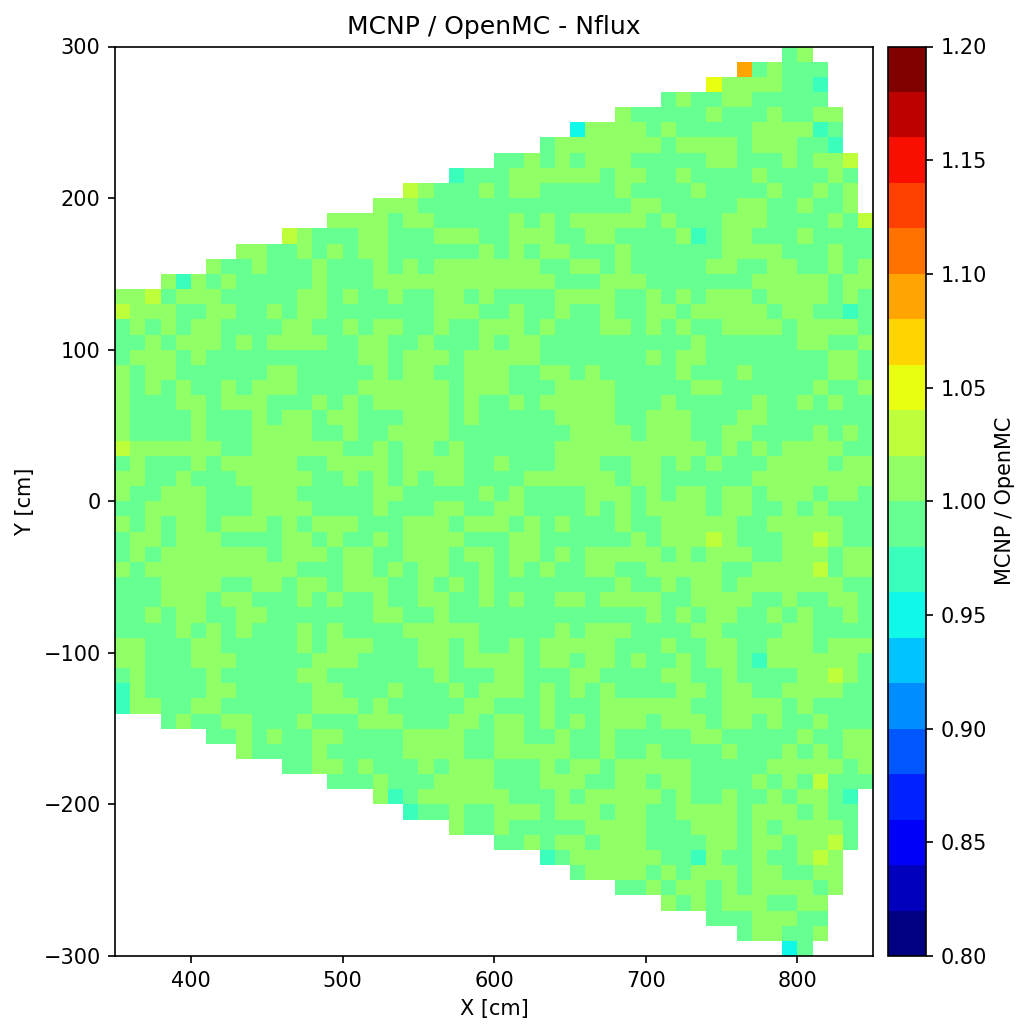
\includegraphics[width=0.54\textwidth]{../fundamental_testing/7224_ss/4/7224_ss_4-Ratio_XY_.png} 
	\hfill 
	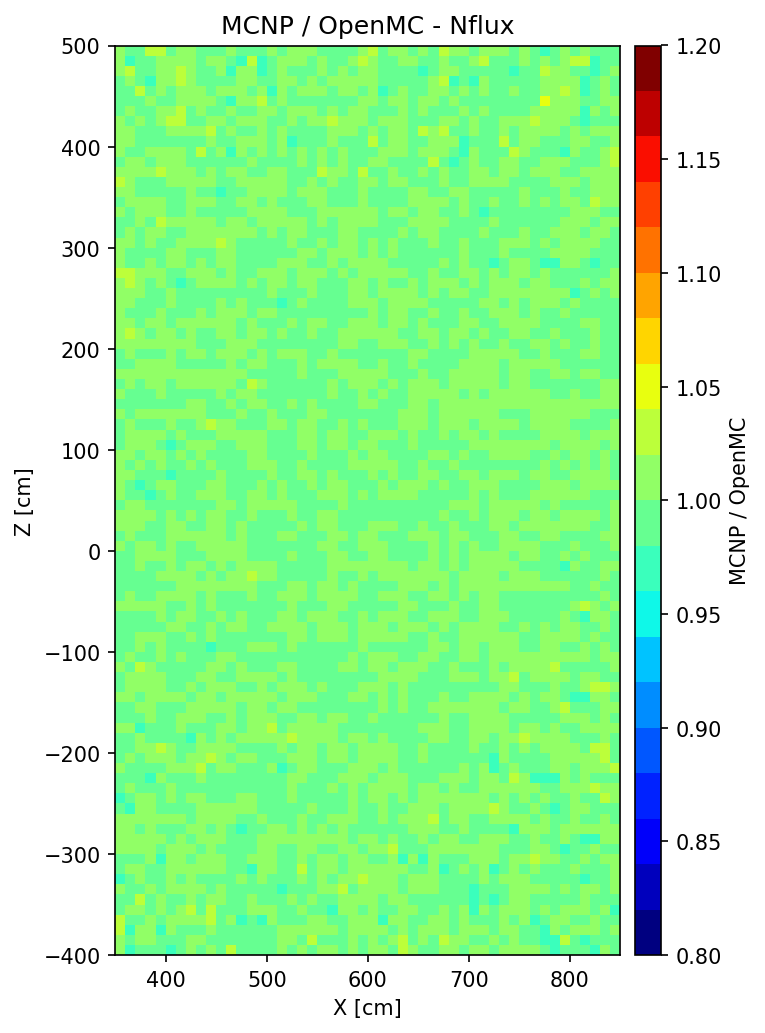
\includegraphics[width=0.44\textwidth]{../fundamental_testing/7224_ss/4/7224_ss_4-Ratio_XZ_.png} 
	\caption{Ratio of MCNP and OpenMC neutron flux over plasma source with reflective boundaries. XY plane (left), XZ plane (right).} 
	\label{fig:7224-4-ratios} 
\end{figure}

\subsubsection{7.2.2.5 Test of conservation of energy for nuclear reaction}
Purpose: To verify the correctness of energy conservation for nuclear reaction.

Test case: The model is a cuboid (50 cm*50 cm*50 cm) with nature iron. The
neutron source is located in the bottom of the cuboid with direction to the negative half
of z axis and mono energy 14MeV. The neutron and photon energy integrated over each
surface of cuboid are counted, as well as heating inside the cuboid.

Test method: Perform the calculation with 100,000,000 particles, and count the
entered and leakage neutron and photon energy independently.

Compare the entered neutron energy A, nuclear heat deposition of neutron and photon
B and the leakage of neutron and photon energy C, then get the subtraction (B+C-A).
The next step, the comparison should be done between the subtraction value and the (n,gamma) 
reaction deposition energy calculated by the code, consider the code passes this test if
the reaction deposition energy has been included in the subtraction value.
\vspace{0.5em}
Problem was setup as described and ran with OpenMC. However the wording of the test is ambigious. It is hard to prove quote: \textit{if the reaction deposition energy has been included in the subtraction value} at the specified 
14 MeV where several reaction (including thresholed) reactions occur that staurate the overall \textit{subtraction value} as it is seen in Figure \ref{fig:7225-1}.
\begin{figure}[H] 
	\centering 
	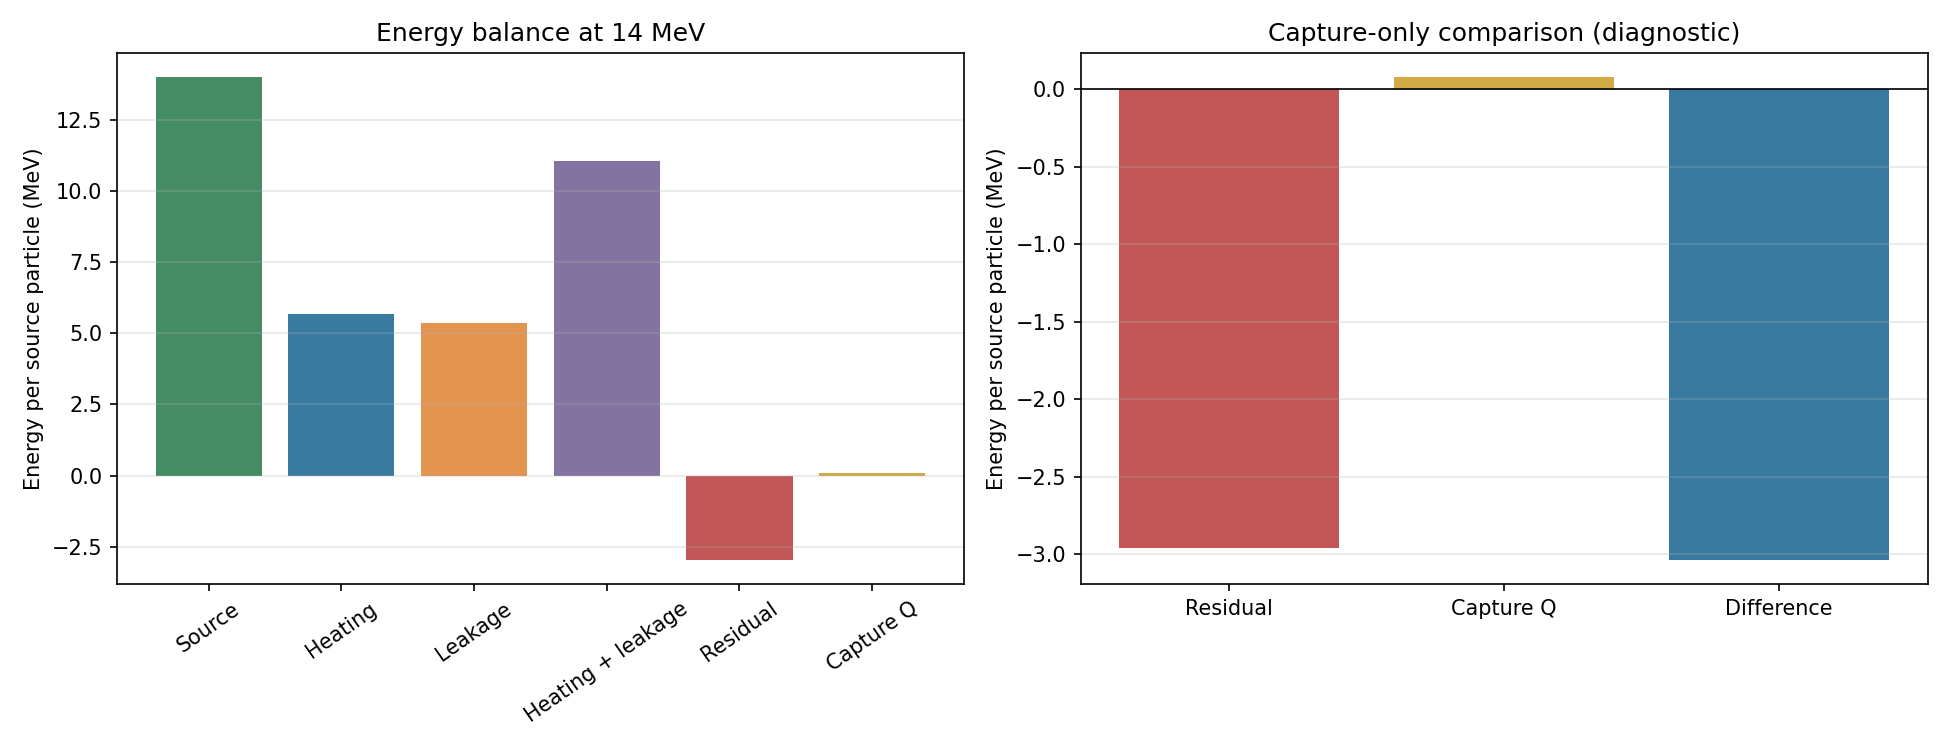
\includegraphics[width=0.95\textwidth]{../fundamental_testing/7225_ce/1/7225_ce_1.png} 
	\caption{Enerergy balance with 14 MeV neutron source. A large residual energy is observed which can be attributed to several reaction channels such as: (n,2n), (n,p), (n,alpha)} 
	\label{fig:7225-1} 
\end{figure}

We propose to ammend the test and run it with 1 MeV neutrons where the energy balance is much simpler and where indeed the subtraction value is close to the capture reaction deposition energy. Results with the 1 MeV source is shown in Figure \ref{fig:7225-2}.  Both tests are performed, but the Summary Results table \ref{tab:fund_res} is linked to the 1 MeV case.
\begin{figure}[H] 
	\centering 
	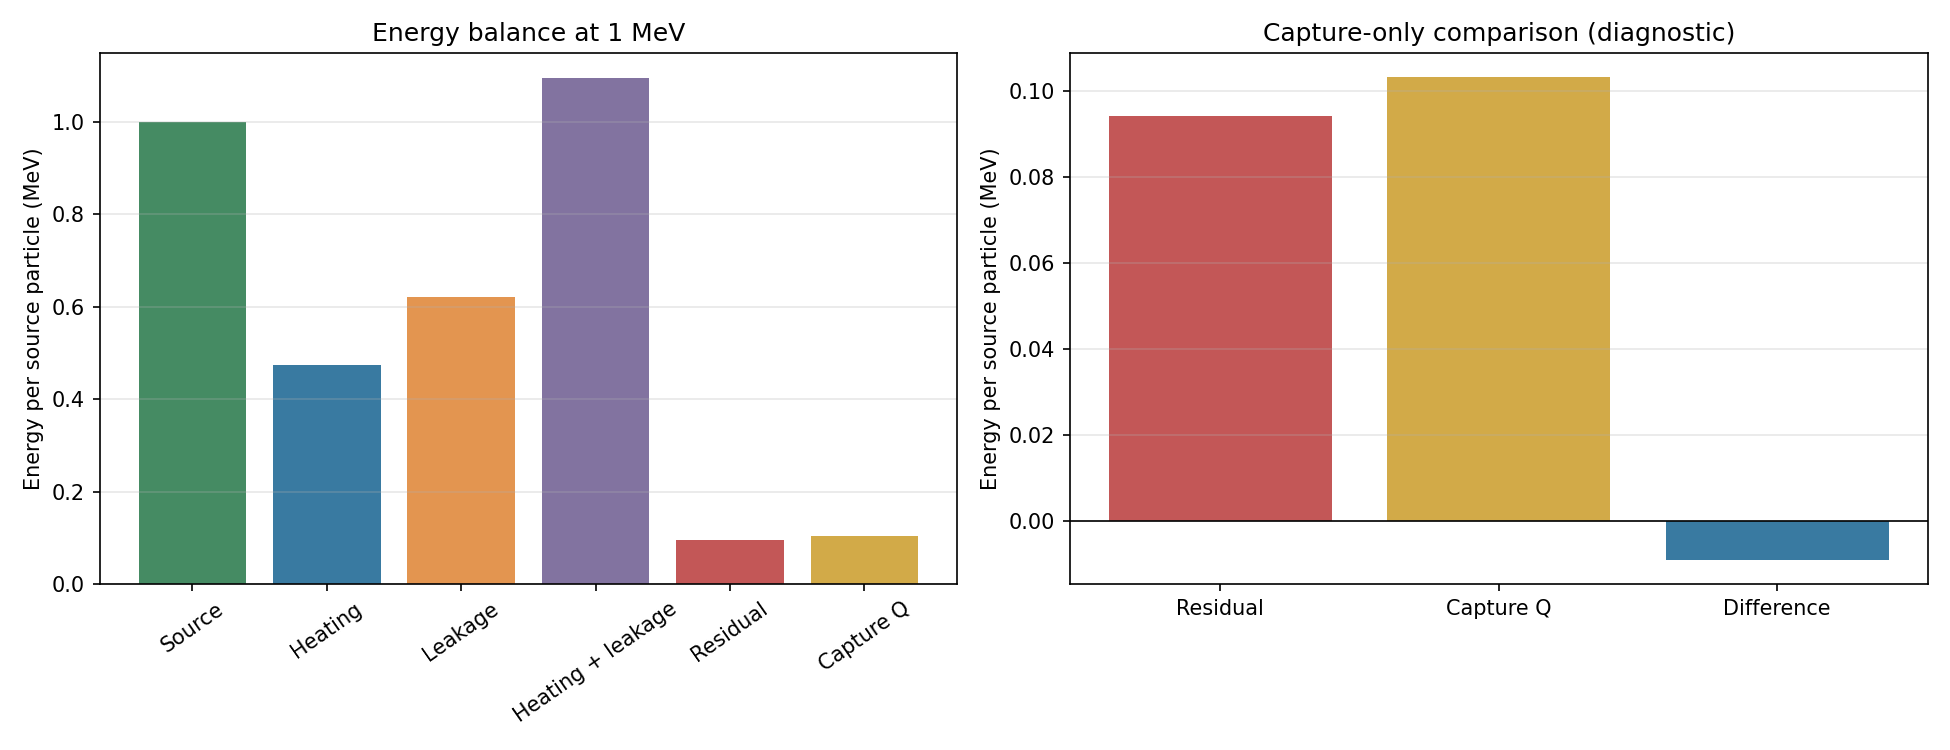
\includegraphics[width=0.95\textwidth]{../fundamental_testing/7225_ce/2/7225_ce_2.png} 
	\caption{Enerergy balance with 14 MeV neutron source. The residual is within uncertainty of the caputre reaction energy depostion.} 
	\label{fig:7225-2} 
\end{figure}

